\documentclass[../Results.tex]{subfiles}
\begin{document}
We construct continuum-free line images by summing over the wavelength range of the emission lines in data cubes and subtracting the underlying continuum component from them. The continuum component is estimated by taking average from another wavelength range without emission nor absorption. We show the results in the left panel of Fig. \ref{overlayspec}. The three contours of different colors representing different emissions show the spatially extended emission of Ly$\alpha$ HeII and CIV with the first contour corresponding to $\rm 2\sigma$ and steps between contours to $\rm 2\sigma$. The background image was taken by Wide Field Camera 3 (WFC3) on Hubble Space Telescope (HST) with F160W filter. Sources labeled from G-1 to G-5 are galaxies at the same redshift ($\rm z \approx 2.3$) with Source-B confirmed by CO (1-0) emission and CO (3-2) emission \citep{emonts2019cold,qiongli2020}. The emitting structure shows Ly$\alpha$ nebula covers all of the marked objects and extends to $\rm 20\arcsec$ which corresponds to 164 kpc. It also shows that the physical projected size of extended HeII and CIV emission reaches to $9 \arcsec$ corresponding to 74 kpc.

Spectra are extracted within aperture with radius of $1.5\arcsec$ centering on the peak of emission (larger than the spatial resolution of KCWI) and shown in the right panel. To determine the redshifts of these widely extended nebulaes, we fit the three emission lines with one-component gaussian function and estimate the wavelength of line centre. The fitted parameters are shown in Tab.\ref{fit_L}. By converting the line width (\AA) to FWHM (km/s) it seems that all of the three emission line have a relatively large FWHM which equals to $\rm FWHM_{Ly}=1225 \ km/s$, $\rm FWHM_{HeII}=1039 \ km/s$ and $\rm FWHM_{CIV}=1786 \ km/s$. This result indicates that there may be extremely violent kinematic activity in the nebula on a physical scale of 100 kpc.

Because the surface brightness (SB) values for both kinematically narrow and broad features would have been either lost in the noise or underestimated in a narrow-band (NB) image with single width of wavelength, we adopt optimally-extract method from \citet{borisova2016ubiquitous} to construct optimally-extracted images which can reach to a larger dynamic range comparing to a standard image. These images are obtained by using a three dimensional segmentation mask (3D mask) which defines a three-dimensional SNR surface in the cube, pixels with values below the SNR threshold are masked and only pixels possessing signal beyond threshold are extracted. Therefore, the signal of each pixel are integrated along a slightly different range in wavelength which allows us to obtain images or spectra with maximal SNR after stacking along spatial axis or spectral axis. In particular, images presented in Fig. \ref{kinematicsmap} (left column) are obtained by using this method after continuum-subtraction and stacking along spectral axis. The three extended emissions are detected at faint levels with 1-$\sigma$ SB of $\rm SB_{Ly}=6.4  \times 10^{-19} \ erg \ s^{-1} \ cm^{2} \ arcsec^{-2}$, $\rm SB_{HeII}= 9.2 \times 10^{-19} \ erg \ s^{-1} \ cm^{2} \ arcsec^{-2}$ and $\rm SB_{CIV}=3.8 \times 10^{-18} \ erg \ s^{-1} \ cm^{2} \ arcsec^{-2}$. 

We also obtain the NB image of H$\rm \alpha$ emission with MOIRCS on Subaru Telescope by using the BrG filter centering on 2.165 $\rm \mu m$ shown in Fig. \ref{H_alpha} (left panel). This result reveals the H$\rm \alpha$ emission on $\rm 14.5\arcsec$ which corresponds to 122 kpc primarily from south to north. The similarity between the shape of H$\alpha$ and Ly$\alpha$ may indicate they have the same powering mechanism. It has a typical surface brightness of $\rm SB_{H\alpha}=1.2 \times 10^{-18} \ erg \ s^{-1} \ cm^{2} \ arcsec^{-2}$ and luminosity of $\rm L_{H\alpha}=2.8 \times 10^{43} \ erg/s$. This extended H$\rm \alpha$ emission beyond 100 kpc is also rarely seen at $\rm z \approx 2$. \citet{Leibler_2018} suggests the ratio between Ly$\rm \alpha$ emission and H$\alpha$ emission can be used as an indicator of the powering mechanism of the nebula. And since Ly$\rm \alpha$ and H$\rm \alpha$ emission have a large overlap area, we then obtain the two-dimensional ratio map and present it in \ref{H_alpha} (right panel). It reveals H$\rm \alpha$ nebula is divided into two parts. The northwest part, "region 1", possesses large ratio but small size and the southwest part, "region 2", has small ratio but large size. "Region 1" shows the ratio decreases from the edge to center with mean value of 0.314 while "Region 2" has the mean value of 6.8. Since "region 1" is compact and overlays on G-1, it is probably emitted from the interstellar medium (ISM) of G-1 instead of the CGM. 


\begin{figure*}
		\centering
		\subfloat[contour]{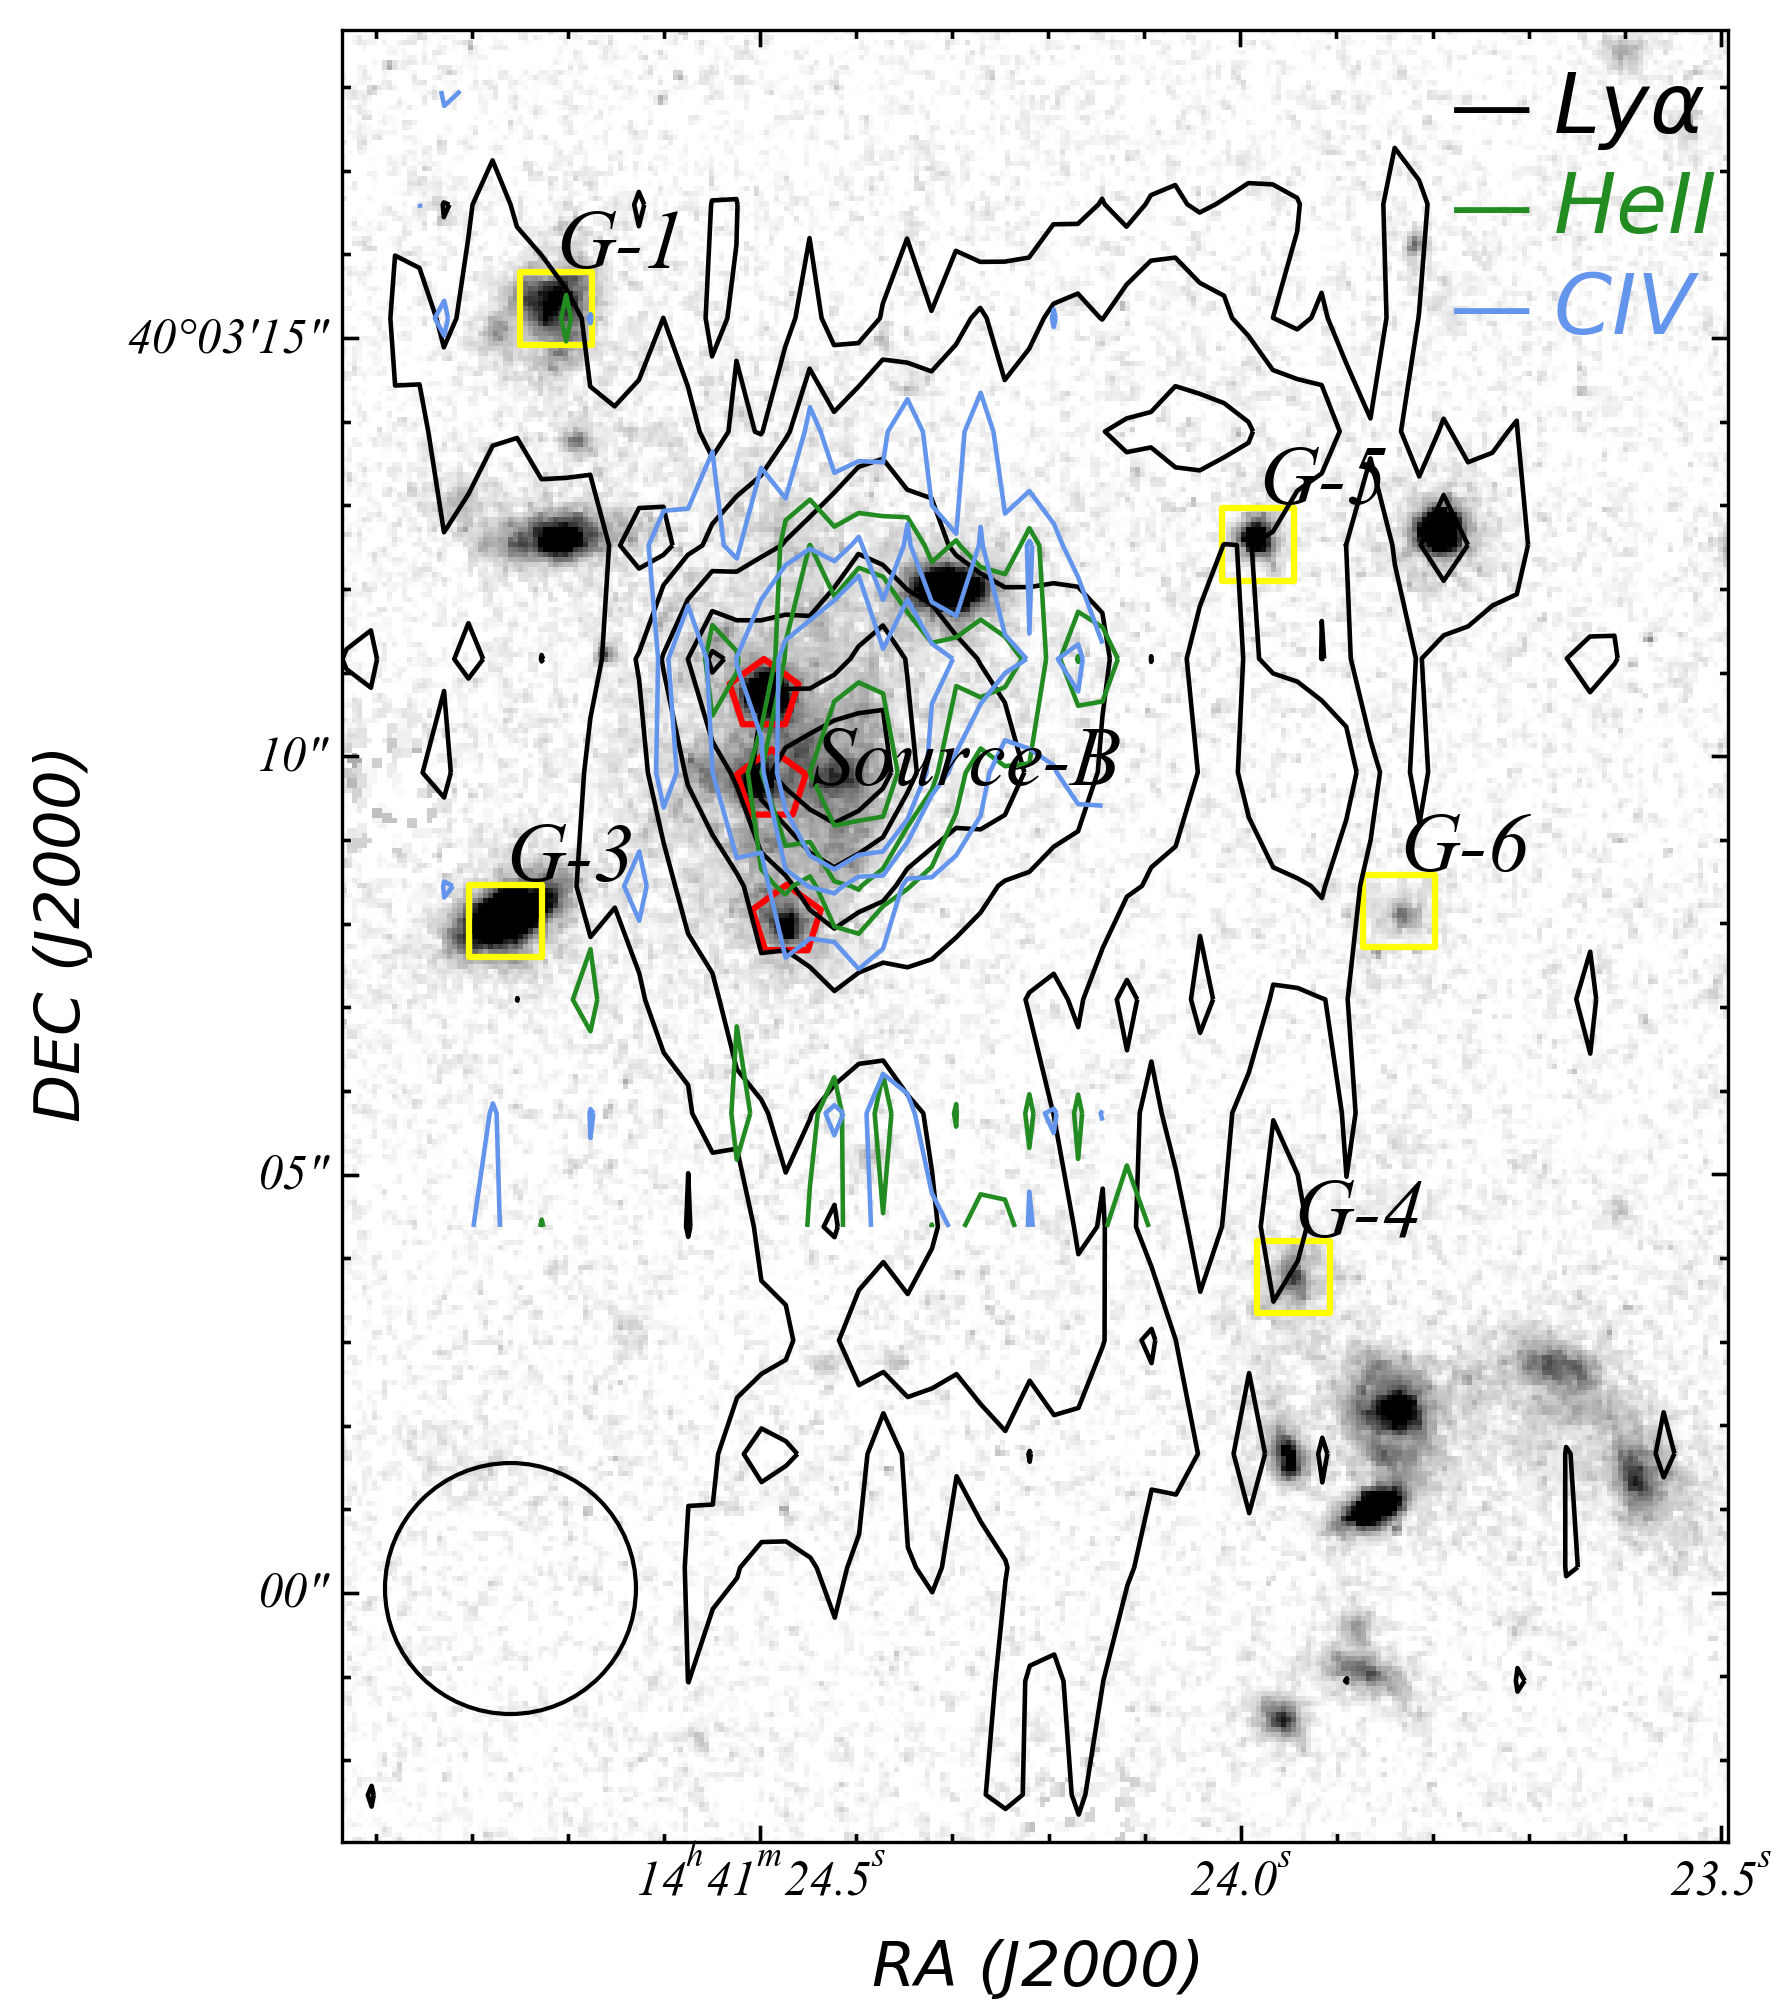
\includegraphics[width=0.5\textwidth]{figs/contour}}
		\subfloat[spectra]{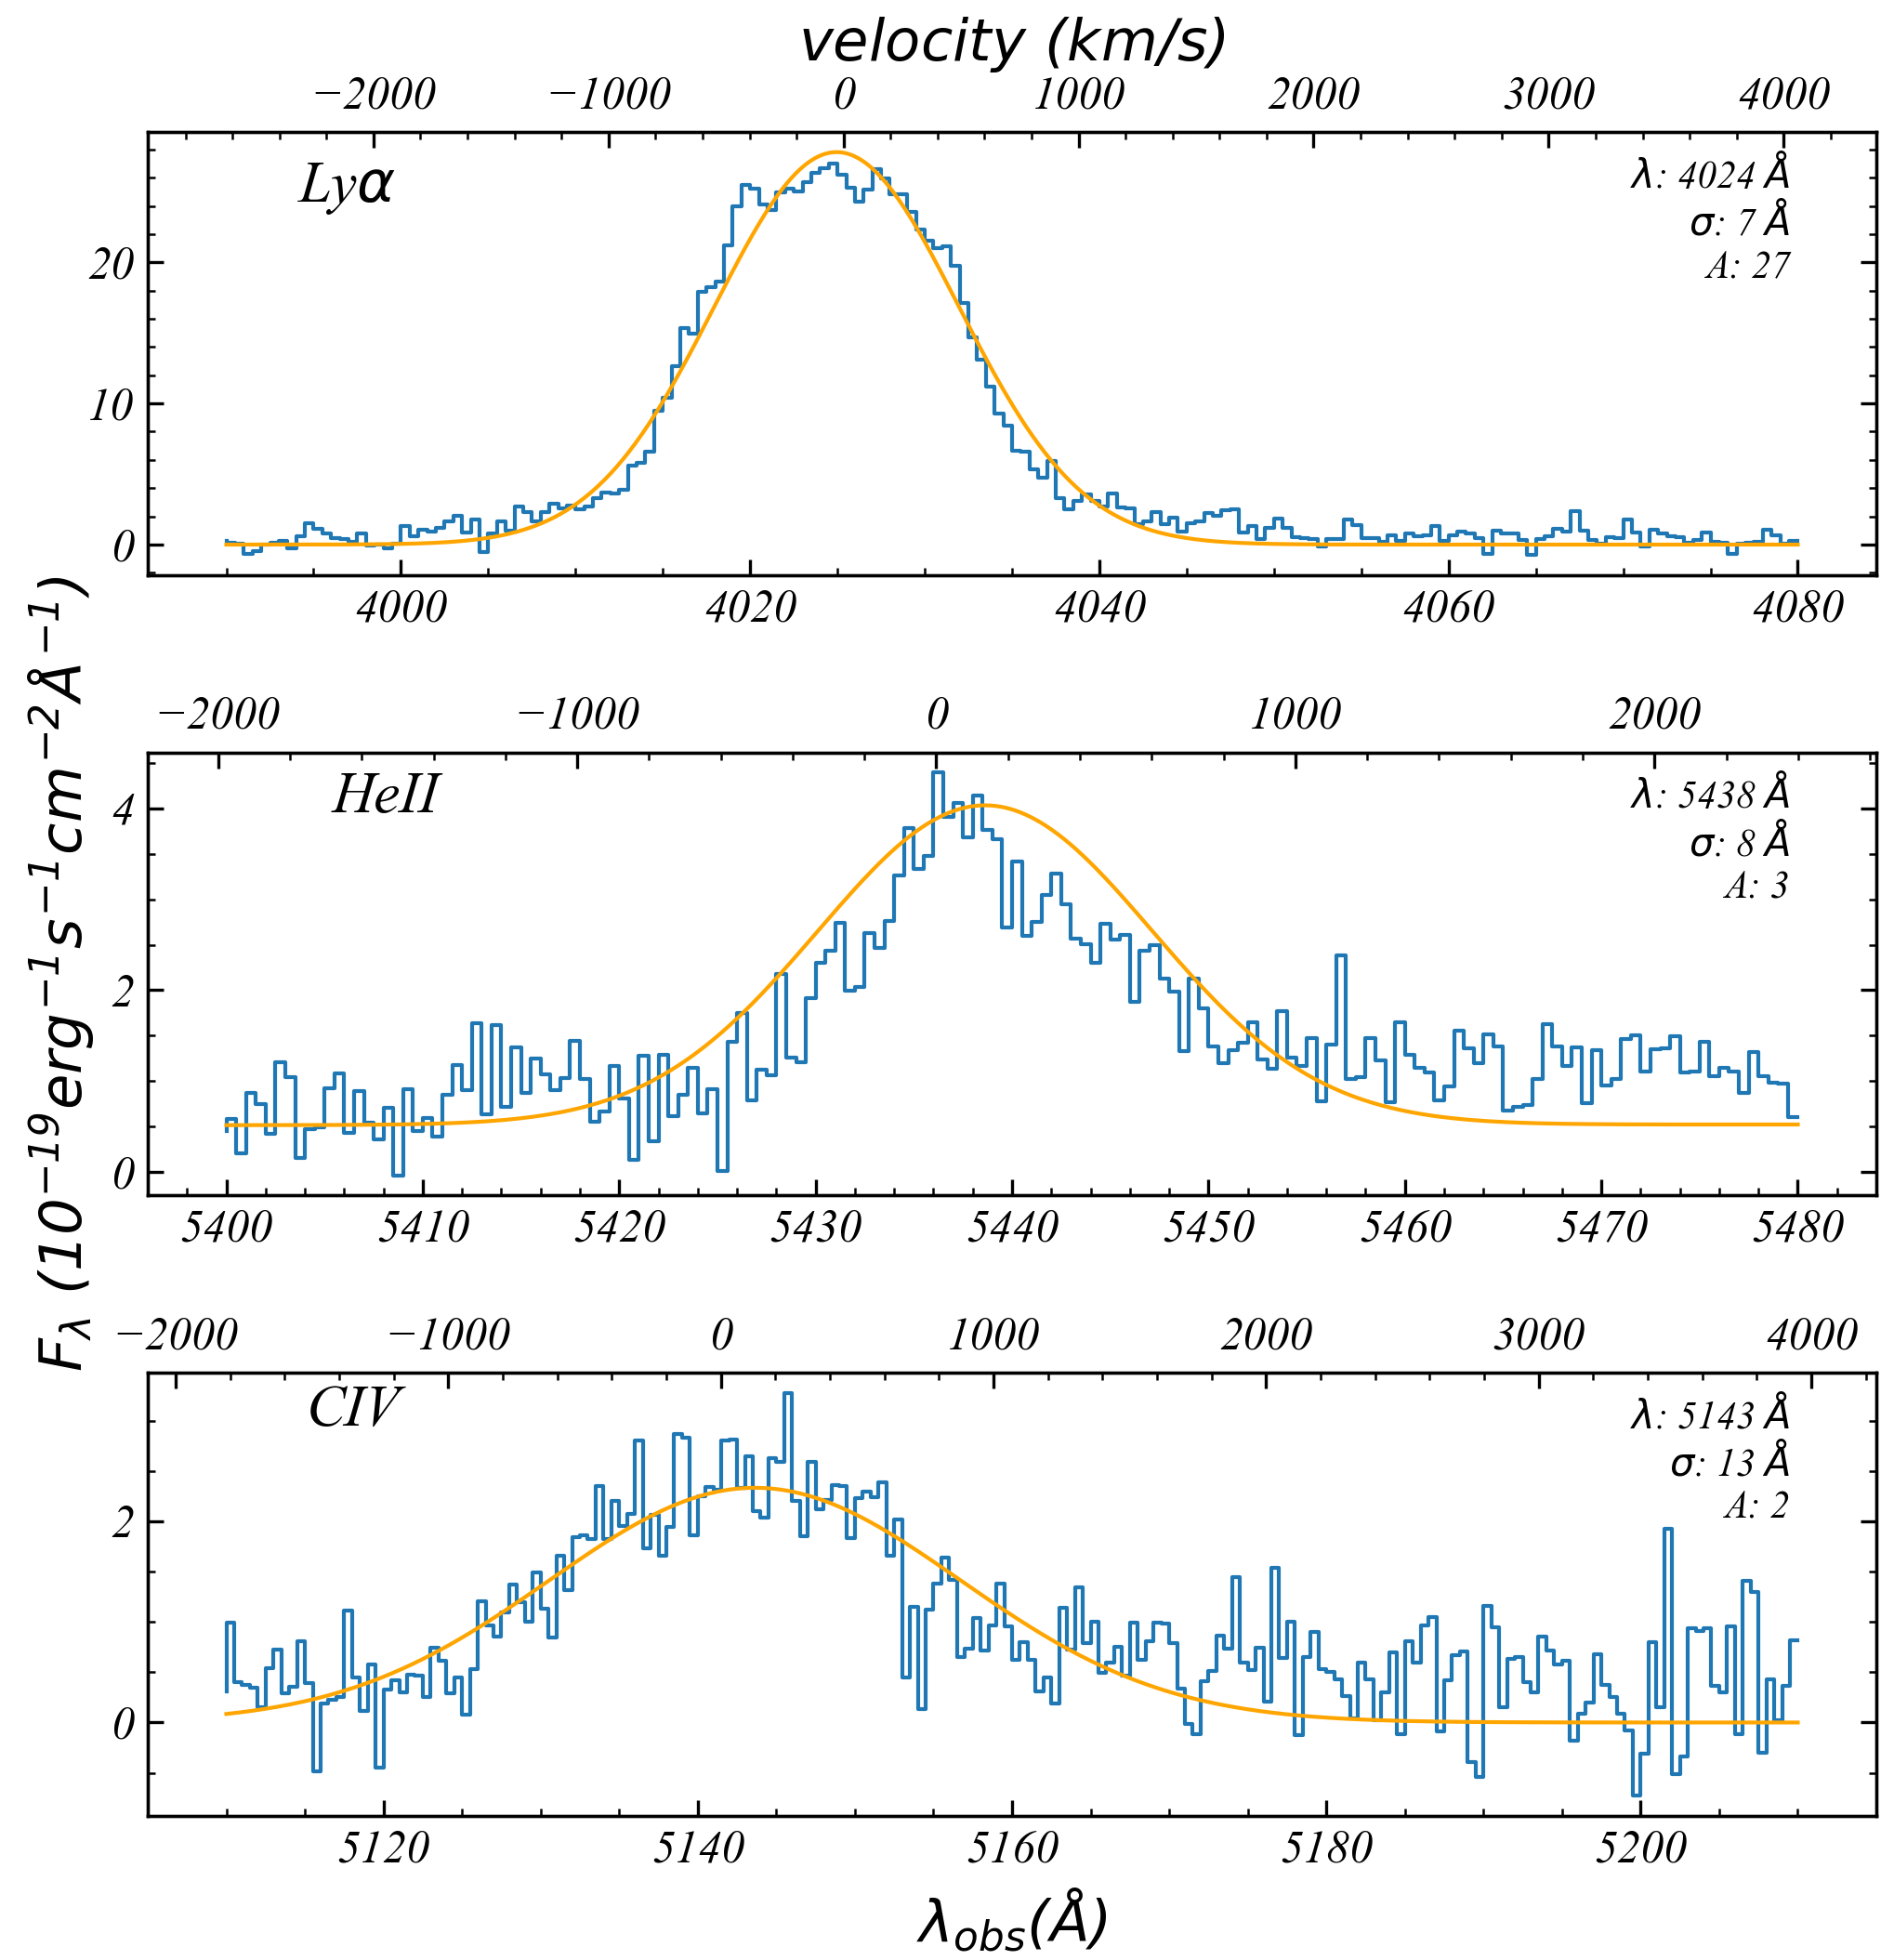
\includegraphics[width=0.5\textwidth]{figs/spectral}}
		\label{overlayspec}
		\caption{Left: HST BW image of MAMMOTH-1 from WFC3 PI: Cai. We overlay the contours of Ly$\rm \alpha$, HeII and CIV emissions on it. Black contours represent Ly$\rm \alpha$, blue contours represent HeII emission while green contours represent CIV emission. We mark source-B with red color and sources at the same redshift with yellow color. The spatial resolution of KCWI is shown in the left bottom. Right: spectra of the 3 emission lines extracted from aperture center on source-B with radius $\rm 1\arcsec$, we fit them with one-component gaussian function.}
\end{figure*}
	\begin{table}[htp]
	\begin{center}
		\begin{tabular}{ccccc}
\hline
\hline
& $\rm \lambda_{c}$(\AA) & $\rm \sigma_{\lambda}$(\AA) & L(erg/s) & redshift \\ \hline
Ly$\alpha$ &   4024  &     7  &   $\rm 2.68 \times 10^{44}$ & 2.310        \\
HeII       &   5438  &     8  &   $\rm 1.97 \times 10^{43}$ & 2.316        \\
CIV        &   5143  &     13 &   $\rm 2.29 \times 10^{43}$ & 2.320        \\ \hline
\end{tabular}
\end{center}
	\caption{}
	\label{fit_L}
	\end{table}

\end{document}